\documentclass[11pt,a4paper]{article}

% --- Essential Packages ---
\usepackage[utf8]{inputenc}
\usepackage[vietnamese,english]{babel}
\usepackage[T5,T1]{fontenc}
\usepackage[margin=1in]{geometry}
\usepackage{graphicx}
\usepackage{booktabs}
\usepackage{amsmath,amssymb}
\usepackage{hyperref}
\usepackage{subcaption}
\usepackage{listings}
\usepackage{xcolor}
\usepackage{float}
\usepackage{microtype}

% Configure graphic search paths for robust local & subfolder compilation
\graphicspath{{../assets/images/}{assets/images/}}

% Hyperlink configuration
\hypersetup{
    colorlinks=true,
    linkcolor=blue!70!black,
    citecolor=red!70!black,
    urlcolor=blue!70!black
}

% Code Listing Configuration
\definecolor{codegreen}{rgb}{0,0.6,0}
\definecolor{codegray}{rgb}{0.5,0.5,0.5}
\definecolor{codepurple}{rgb}{0.58,0,0.82}
\definecolor{backcolour}{rgb}{0.97,0.97,0.97}

\lstdefinestyle{mystyle}{
    backgroundcolor=\color{backcolour},   
    commentstyle=\color{codegreen}\itshape,
    keywordstyle=\color{blue}\bfseries,
    numberstyle=\tiny\color{codegray},
    stringstyle=\color{codepurple},
    basicstyle=\ttfamily\footnotesize,
    breakatwhitespace=false,         
    breaklines=true,                 
    captionpos=b,                    
    keepspaces=true,                 
    numbers=left,                    
    numbersep=6pt,                  
    showspaces=false,                
    showstringspaces=false,
    showtabs=false,                  
    tabsize=2,
    frame=single,
    rulecolor=\color{black!20}
}
\lstset{style=mystyle}

% Thiết lập ngôn ngữ tiếng Việt làm ngôn ngữ chính
\selectlanguage{vietnamese}

% --- Document Metadata ---
\title{\textbf{Phân tích Cảm xúc trên Tập Dữ liệu Đánh giá Phim IMDB sử dụng Mạng Nơ-ron Hồi quy (Vanilla RNN)}}
\author{[Tên Tác Giả]}
\date{\today}

\begin{document}

\maketitle

\begin{abstract}
Báo cáo này trình bày một nghiên cứu khoa học và thực nghiệm toàn diện về việc huấn luyện một Mạng Nơ-ron Hồi quy Cơ bản (Vanilla SimpleRNN) từ đầu (from scratch) cho bài toán phân loại cảm xúc nhị phân trên tập dữ liệu đánh giá phim quy mô lớn IMDB. Dữ liệu văn bản tuần tự đặt ra các thách thức đặc thù trong học máy do tính phụ thuộc thời gian và cấu trúc cú pháp phi dừng. Chúng tôi xây dựng một quy trình học sâu hoàn chỉnh khép kín bao gồm: loại bỏ thẻ HTML, chuẩn hóa ký tự bằng biểu thức chính quy (regex), số hóa token thông qua tập từ vựng thích ứng gồm 1.000 từ, nhúng từ không gian dày đặc (dense word embeddings), và khối nơ-ron hồi quy kết hợp với tầng phân loại đầu ra sử dụng hàm kích hoạt sigmoid. Trải qua 10 epoch huấn luyện trên 25.000 mẫu đánh giá và kiểm chuẩn (validation) trên 25.000 mẫu đánh giá độc lập, mạng nơ-ron thể hiện sự hội tụ đơn điệu rõ rệt, cải thiện từ độ mất mát huấn luyện ban đầu là 0,6351 (độ chính xác 63,19\%) xuống mức 0,3117 (độ chính xác 86,92\%). Trên tập kiểm thử độc lập (test set), mô hình đạt độ chính xác phân loại (accuracy) 83,66\%, độ chính xác dương tính (precision) 80,00\%, độ bao phủ (recall) 89,69\%, điểm $F_1$ đạt 84,57\%, và diện tích dưới đường cong đặc trưng hoạt động của bộ thu (ROC-AUC) đạt 0,9193. Báo cáo cung cấp trực quan hóa chi tiết tiến trình huấn luyện, phân tích ma trận nhầm lẫn (confusion matrix), và xem xét các cơ chế sai số do hiện tượng triệt tiêu đạo hàm (vanishing gradient) cố hữu trong quá trình lan truyền ngược qua thời gian (BPTT) trên chuỗi dài.
\end{abstract}

\vspace{0.5em}
\noindent\textbf{Từ khóa:} Phân tích Cảm xúc, Xử lý Ngôn ngữ Tự nhiên, Mạng Nơ-ron Hồi quy, SimpleRNN, Học Sâu, TensorFlow/Keras, IMDB Benchmark.

\newpage
\tableofcontents
\newpage

% =========================================================================
\section{Giới thiệu}
% =========================================================================

\subsection{Động lực Nghiên cứu}
Phân tích cảm xúc (Sentiment Analysis)—quá trình tự động trích xuất và phân loại các quan điểm chủ quan cùng xu hướng cảm xúc từ ngôn ngữ tự nhiên phi cấu trúc—là một trụ cột nền tảng của ngành xử lý ngôn ngữ tự nhiên và trí tuệ ra quyết định hiện đại. Trong kỷ nguyên số ngày nay, hàng triệu đánh giá của người dùng, bài đăng trên mạng xã hội và phản hồi về sản phẩm được phát hành mỗi ngày. Việc khai thác các thông tin hữu ích này theo phương pháp thủ công là hoàn toàn bất khả thi về mặt chi phí và nhân lực. Các mô hình chuỗi tự động cho phép các tổ chức đánh giá mức độ đón nhận của công chúng, theo dõi mức độ hài lòng của khách hàng và dự báo xu hướng thương mại trên quy mô lớn.

Các cách tiếp cận truyền thống dựa trên túi từ (Bag-of-Words - BoW), ví dụ như mô hình TF-IDF kết hợp với Naive Bayes hoặc Hồi quy Logistic, thường xem văn bản như những tập hợp từ ngẫu nhiên không có thứ tự. Mặc dù có ưu thế về chi phí tính toán thấp, các biểu diễn này hoàn toàn triệt tiêu trật tự từ tuần tự, hệ thống phân cấp cú pháp và ngữ cảnh ngữ nghĩa tầm xa. Mạng Nơ-ron Hồi quy (Recurrent Neural Networks - RNN) giải quyết triệt để hạn chế này bằng cách duy trì một vector trạng thái nội bộ liên tục được cập nhật qua từng bước thời gian, giúp mạng học được các biểu diễn cấp câu dựa trên tiến trình diễn đạt tuần tự của ngôn ngữ.

\subsection{Phát biểu Bài toán}
Cho một văn bản đánh giá tự nhiên bất kỳ $x = (w_1, w_2, \dots, w_T)$ bao gồm chuỗi $T$ từ (tokens), mục tiêu là suy luận ra một nhãn phân loại nhị phân:
\begin{equation}
y \in \{0, 1\}
\end{equation}
trong đó $y = 1$ đại diện cho cảm xúc tích cực (positive) và $y = 0$ đại diện cho cảm xúc tiêu cực (negative). Mô hình cần học một hàm ánh xạ quy nạp $\hat{y} = f_\theta(x) \in [0, 1]$ được tham số hóa bởi tập trọng số $\theta$, nhằm cực tiểu hóa sai số phân loại đồng thời đạt khả năng tổng quát hóa cao trên các mẫu văn bản chưa từng xuất hiện trong quá trình huấn luyện.

\subsection{Mục tiêu Đề tài}
Các mục tiêu trọng tâm của nghiên cứu này bao gồm:
\begin{enumerate}
    \item Thiết kế và xây dựng một quy trình học sâu khép kín (end-to-end) cho bài toán phân loại chuỗi nhị phân sử dụng nền tảng TensorFlow và Keras.
    \item Hiện thực hóa một đường ống chuẩn hóa văn bản và số hóa token tùy biến, có khả năng chuyển đổi trực tiếp văn bản thô phi cấu trúc thành các tensor số học có kích thước giới hạn.
    \item Thiết lập, huấn luyện và kiểm chuẩn kiến trúc Vanilla SimpleRNN vận hành trên không gian nhúng từ dày đặc (dense embeddings).
    \item Theo dõi và ghi nhận chặt chẽ tiến trình huấn luyện qua 10 epoch, đánh giá xu hướng cực tiểu hóa hàm mất mát, quỹ đạo độ chính xác và các dấu hiệu tiềm ẩn của hiện tượng quá khớp (overfitting) hoặc chưa khớp (underfitting).
    \item Đánh giá hiệu năng tổng quát hóa trên tập kiểm thử cân bằng gồm 25.000 mẫu thông qua các thang đo toàn diện, bao gồm Ma trận Nhầm lẫn và đường cong Đặc trưng Hoạt động của Bộ thu (ROC).
    \item Thực hiện phân tích định tính các trường hợp phân loại sai nhằm làm sáng tỏ các cơ chế gây lỗi trong thực tế.
\end{enumerate}

\subsection{Các Đóng góp Chính}
Các đóng góp kỹ thuật đạt được trong công trình này gồm có:
\begin{itemize}
    \item \textbf{Đường ống Vận hành Nội bộ Khép kín:} Khai thác trọn vẹn tập dữ liệu 50.000 đánh giá IMDB lưu trữ cục bộ mà không phụ thuộc vào kết nối mạng tải ngoài khi thực thi.
    \item \textbf{Kiến trúc Tiền xử lý Tích hợp:} Nhúng trực tiếp tầng chuẩn hóa và vector hóa văn bản vào trong đồ thị tính toán của mô hình, hỗ trợ suy luận trực tiếp từ chuỗi ký tự thô mà không cần bước tiền xử lý tách rời.
    \item \textbf{Cơ sở Dữ liệu Thực nghiệm Xác thực:} Tạo lập các biểu đồ tiến trình huấn luyện, ma trận nhầm lẫn, đường cong ROC và các bảng thống kê số liệu thực nghiệm chính xác, có khả năng tái lập hoàn toàn.
    \item \textbf{Chẩn đoán Lý thuyết Chuyên sâu:} Kết nối hiện tượng bão hòa hiệu năng thực nghiệm với cơ chế triệt tiêu đạo hàm trong thuật toán Lan truyền Ngược qua Thời gian (BPTT).
\end{itemize}

\subsection{Cấu trúc Báo cáo}
Phần còn lại của báo cáo được bố cục như sau: Mục~\ref{sec:theory} trình bày nền tảng lý thuyết của mô hình chuỗi và tính toán hồi quy trong Vanilla RNN. Mục~\ref{sec:dataset} chi tiết hóa thống kê tập dữ liệu, phân tích khám phá (EDA) và quy trình tiền xử lý. Mục~\ref{sec:architecture} mô tả cấu trúc mạng và thông số từng tầng. Mục~\ref{sec:setup} trình bày thiết lập thực nghiệm, môi trường tính toán và các chỉ số đo lường. Mục~\ref{sec:results} công bố kết quả thực nghiệm chi tiết về tiến trình huấn luyện và đánh giá trên tập kiểm thử. Mục~\ref{sec:discussion} thảo luận về các phát hiện thực nghiệm và giới hạn của kiến trúc. Mục~\ref{sec:conclusion} tổng kết nghiên cứu và đề xuất hướng mở rộng. Các đoạn mã nguồn tiêu biểu được đính kèm tại Phụ lục~\ref{sec:appendix}.

% =========================================================================
\section{Cơ sở Lý thuyết}
\label{sec:theory}
% =========================================================================

\subsection{Phân tích Cảm xúc}
Phân tích cảm xúc thực hiện ánh xạ các chuỗi ký hiệu từ vựng có độ dài thay đổi sang một không gian xác suất liên tục. Trong phân loại đánh giá phim ảnh, mô hình phải phân tách được các cấu trúc ngôn ngữ phức tạp như phủ định (ví dụ: ``not good''), liên từ tương phản (ví dụ: ``the acting was decent, but the script was terrible''), cũng như hiện tượng châm biếm và mỉa mai.

\subsection{Khái niệm Cơ bản về Mạng Nơ-ron}
Mạng nơ-ron truyền thẳng (Feedforward Neural Networks) xử lý một vector đầu vào $x \in \mathbb{R}^D$ qua các phép biến đổi affine kết hợp với các hàm kích hoạt phi tuyến:
\begin{equation}
z = Wx + b, \quad a = \phi(z)
\end{equation}
trong đó $W$ là ma trận trọng số, $b$ là vector độ lệch (bias), và $\phi(\cdot)$ là hàm kích hoạt phi tuyến (như ReLU hoặc $\tanh$). Trong mạng truyền thẳng thông thường, các mẫu dữ liệu đầu vào được giả định là độc lập và phân phối đồng nhất (i.i.d.), khiến chúng không phù hợp một cách tự nhiên cho các chuỗi dữ liệu có mối tương quan chặt chẽ về mặt thời gian.

\subsection{Mạng Nơ-ron Hồi quy (Recurrent Neural Networks - RNN)}
Mạng Nơ-ron Hồi quy xử lý chuỗi đầu vào $(x_1, x_2, \dots, x_T)$ bằng cách duy trì một trạng thái ẩn hồi quy $h_t \in \mathbb{R}^H$. Tại mỗi bước thời gian rời rạc $t$, trạng thái ẩn được cập nhật phụ thuộc vào vector đầu vào hiện tại $x_t \in \mathbb{R}^D$ và trạng thái ẩn liền trước $h_{t-1} \in \mathbb{R}^H$:
\begin{equation}
h_t = \tanh(W_{hh} h_{t-1} + W_{xh} x_t + b_h)
\label{eq:rnn_hidden}
\end{equation}
trong đó:
\begin{itemize}
    \item $W_{xh} \in \mathbb{R}^{H \times D}$ đại diện cho ma trận trọng số chuyển tiếp từ đầu vào sang trạng thái ẩn.
    \item $W_{hh} \in \mathbb{R}^{H \times H}$ đại diện cho ma trận trọng số chuyển tiếp hồi quy giữa các trạng thái ẩn.
    \item $b_h \in \mathbb{R}^H$ là vector độ lệch của trạng thái ẩn.
    \item $\tanh(\cdot)$ cung cấp phép kích hoạt phi tuyến ánh xạ các giá trị trạng thái ẩn vào khoảng $(-1, 1)$.
\end{itemize}

Đối với bài toán phân loại chuỗi nhiều-sang-một (many-to-one), mạng nơ-ron duyệt qua toàn bộ chuỗi đến bước thời gian cuối cùng $T$. Vector tổng hợp $h_T$ sau đó được chiếu tới một giá trị vô hướng duy nhất thông qua tầng Dense với hàm kích hoạt sigmoid:
\begin{equation}
\hat{y} = \sigma(W_{hy} h_T + b_y) = \frac{1}{1 + e^{-(W_{hy} h_T + b_y)}}
\label{eq:rnn_output}
\end{equation}
trong đó $W_{hy} \in \mathbb{R}^{1 \times H}$ và $b_y \in \mathbb{R}$.

\begin{figure}[H]
\centering
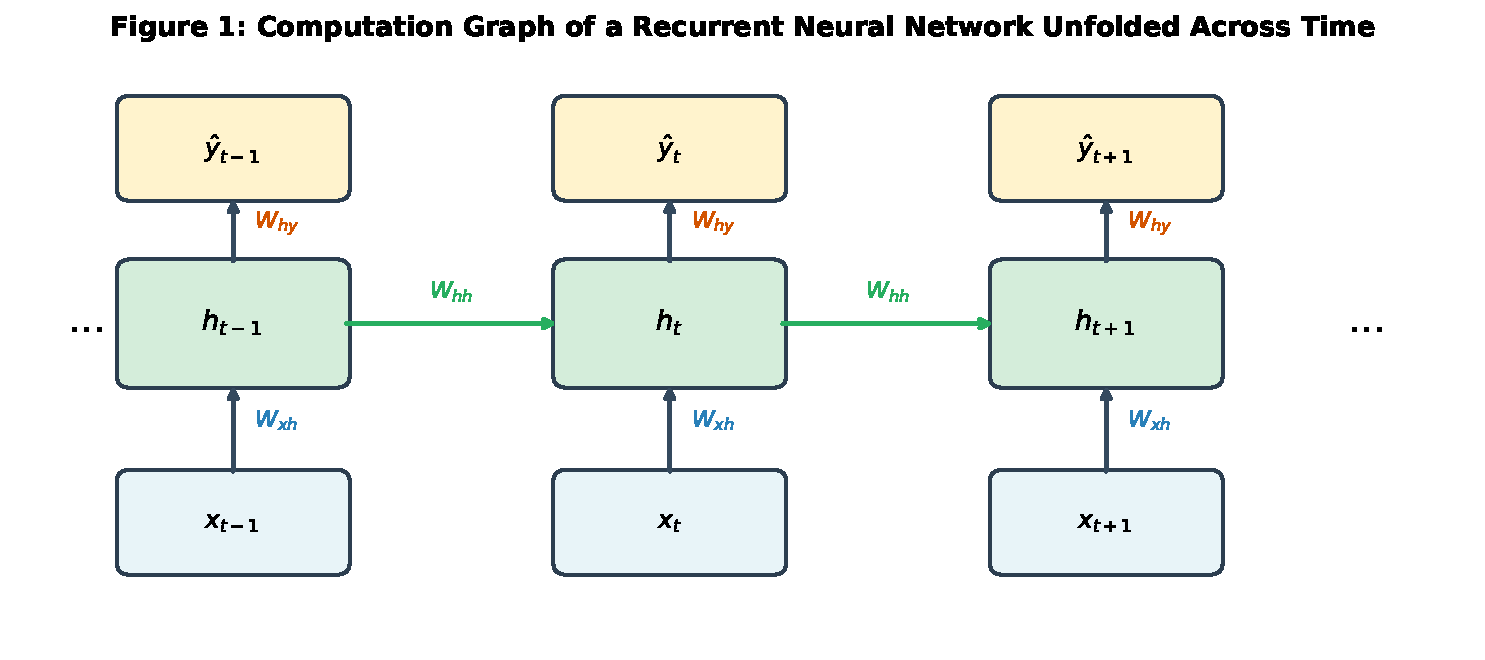
\includegraphics[width=0.88\textwidth]{fig1_rnn_unfolded.pdf}
\caption{Đồ thị tính toán của Mạng Nơ-ron Hồi quy cơ bản (Vanilla RNN) được trải phẳng theo các bước thời gian $t-1$, $t$, và $t+1$. Các ma trận trọng số $W_{xh}$, $W_{hh}$, và $W_{hy}$ được chia sẻ đồng nhất qua tất cả các bước thời gian.}
\label{fig:unfolded_rnn}
\end{figure}

Hình~\ref{fig:unfolded_rnn} minh họa đồ thị tính toán của một RNN được trải phẳng theo thời gian. Đặc tính kiến trúc cốt lõi ở đây là \textit{chia sẻ tham số} (parameter sharing): các ma trận $W_{xh}$ và $W_{hh}$ giữ nguyên giá trị tại mọi bước thời gian, giúp mô hình có khả năng xử lý các chuỗi có độ dài tùy ý mà không làm gia tăng số lượng tham số cần học.

\subsection{Lan truyền Ngược qua Thời gian (BPTT)}
Các tham số của mô hình được tối ưu hóa thông qua thuật toán Lan truyền Ngược qua Thời gian (Backpropagation Through Time - BPTT). Hàm mất mát tổng thể $\mathcal{L}$ được tính tại bước kết thúc chuỗi $T$. Áp dụng quy tắc đạo hàm theo chuỗi (chain rule), đạo hàm của hàm mất mát đối với ma trận trọng số hồi quy $W_{hh}$ được mở rộng thành tổng đóng góp qua từng bước thời gian:
\begin{equation}
\frac{\partial \mathcal{L}}{\partial W_{hh}} = \sum_{t=1}^{T} \frac{\partial \mathcal{L}}{\partial \hat{y}} \frac{\partial \hat{y}}{\partial h_T} \frac{\partial h_T}{\partial h_t} \frac{\partial h_t}{\partial W_{hh}}
\end{equation}
Hệ số ma trận Jacobian $\frac{\partial h_T}{\partial h_t}$ có thể phân rã thành tích liên tiếp của các ma trận Jacobian trung gian:
\begin{equation}
\frac{\partial h_T}{\partial h_t} = \prod_{k=t+1}^{T} \frac{\partial h_k}{\partial h_{k-1}} = \prod_{k=t+1}^{T} \operatorname{diag}\left(1 - \tanh^2(\cdot)\right) W_{hh}^T
\label{eq:jacobian_product}
\end{equation}

Phương trình~\eqref{eq:jacobian_product} làm sáng tỏ điểm yếu cố hữu của Vanilla RNN. Nếu giá trị riêng lớn nhất của ma trận $W_{hh}$ nhỏ hơn 1 ($\lambda_{\max} < 1$) và đạo hàm của hàm $\tanh$ thỏa mãn $|1 - \tanh^2(z)| \le 1$, tích liên tiếp của các ma trận này sẽ suy giảm theo hàm mũ khi khoảng cách thời gian $(T - t)$ tăng lên:
\begin{equation}
\lim_{(T - t) \to \infty} \left\| \frac{\partial h_T}{\partial h_t} \right\| \to 0
\end{equation}
Đây chính là hiện tượng \textbf{Triệt tiêu Đạo hàm (Vanishing Gradient Problem)}. Hậu quả là tín hiệu gradient xuất phát từ bước $t = T$ sẽ tiêu biến hoàn toàn và không thể cập nhật hiệu quả các trọng số đối với các từ xuất hiện ở đầu chuỗi ($t \ll T$). Ngược lại, nếu các giá trị riêng vượt quá 1 mà không có cơ chế điều hòa, gradient có thể bùng nổ ($\to \infty$), gây mất ổn định số học.

\subsection{Nhúng Từ (Word Embeddings)}
Phương pháp mã hóa one-hot biểu diễn từ ngữ dưới dạng các vector thưa thớt, trực giao trong không gian có số chiều bằng kích thước từ vựng $|V|$, hoàn toàn làm mất đi quan hệ tương đồng ngữ nghĩa (tức là $\mathbf{e}_{\text{good}}^T \mathbf{e}_{\text{great}} = 0$). Tầng Nhúng từ (Embedding Layer) ánh xạ các chỉ số token rời rạc $i \in \{0, \dots, |V|-1\}$ thành các vector liên tục dày đặc $x_t \in \mathbb{R}^D$ với số chiều nhỏ hơn rất nhiều ($D \ll |V|$):
\begin{equation}
x_t = E \cdot \mathbf{one\_hot}(i)
\end{equation}
trong đó $E \in \mathbb{R}^{|V| \times D}$ là bảng tra cứu nhúng từ có thể huấn luyện được. Trong quá trình học, khoảng cách hình học giữa các vector trong không gian nhúng sẽ tự động sắp xếp tương ứng với mối liên hệ cú pháp và ngữ nghĩa của các từ.

\subsection{Hàm Mất mát Entropy Chéo Nhị phân}
Vì giá trị đầu ra $\hat{y}_i \in [0, 1]$ mô hình hóa phân phối xác suất Bernoulli $P(y_i = 1 \mid x_i)$, các trọng số mạng được ước lượng thông qua nguyên lý hợp lý cực đại (maximum likelihood), được chuẩn hóa thành hàm mất mát Entropy Chéo Nhị phân (Binary Cross-Entropy - BCE):
\begin{equation}
\mathcal{L}(\theta) = -\frac{1}{N}\sum_{i=1}^{N} \left[ y_i \log(\hat{y}_i) + (1 - y_i)\log(1 - \hat{y}_i) \right]
\label{eq:bce_loss}
\end{equation}
với $N$ là kích thước batch mẫu, $y_i \in \{0, 1\}$ là nhãn thực tế, và $\hat{y}_i$ là xác suất dự đoán của mô hình.

% =========================================================================
\section{Tập Dữ liệu và Quy trình Tiền xử lý}
\label{sec:dataset}
% =========================================================================

\subsection{Mô tả Tập Dữ liệu}
Tập dữ liệu thực nghiệm được sử dụng là Large Movie Review Dataset (IMDB), một bộ dữ liệu tiêu chuẩn gồm 50.000 đánh giá phim phân cực mạnh. Dữ liệu được chia đều thành 25.000 đánh giá cho tập huấn luyện và 25.000 đánh giá cho tập kiểm thử, đảm bảo tỷ lệ cân bằng tuyệt đối 50\% nhãn tích cực và 50\% nhãn tiêu cực trên cả hai phân vùng, như được thống kê trong Bảng~\ref{tab:dataset_stats}.

\begin{table}[H]
\centering
\begin{tabular}{lrrr}
\toprule
\textbf{Phân vùng} & \textbf{Đánh giá Tiêu cực ($y=0$)} & \textbf{Đánh giá Tích cực ($y=1$)} & \textbf{Tổng Số lượng} \\
\midrule
Tập Huấn luyện ($D_{\text{train}}$) & 12.500 & 12.500 & 25.000 \\
Tập Kiểm thử ($D_{\text{test}}$)     & 12.500 & 12.500 & 25.000 \\
\midrule
\textbf{Toàn bộ Tập dữ liệu}        & \textbf{25.000} & \textbf{25.000} & \textbf{50.000} \\
\bottomrule
\end{tabular}
\caption{Thống kê phân chia tập dữ liệu và phân bố nhãn lớp của IMDB.}
\label{tab:dataset_stats}
\end{table}

\subsection{Phân tích Khám phá Dữ liệu (EDA)}
Trước khi tiến hành vector hóa, các phân tích thống kê mô tả đã được thực hiện trên tập văn bản thô. Hình~\ref{fig:eda_class} khẳng định tính cân bằng tuyệt đối giữa hai lớp cảm xúc.

\begin{figure}[H]
\centering
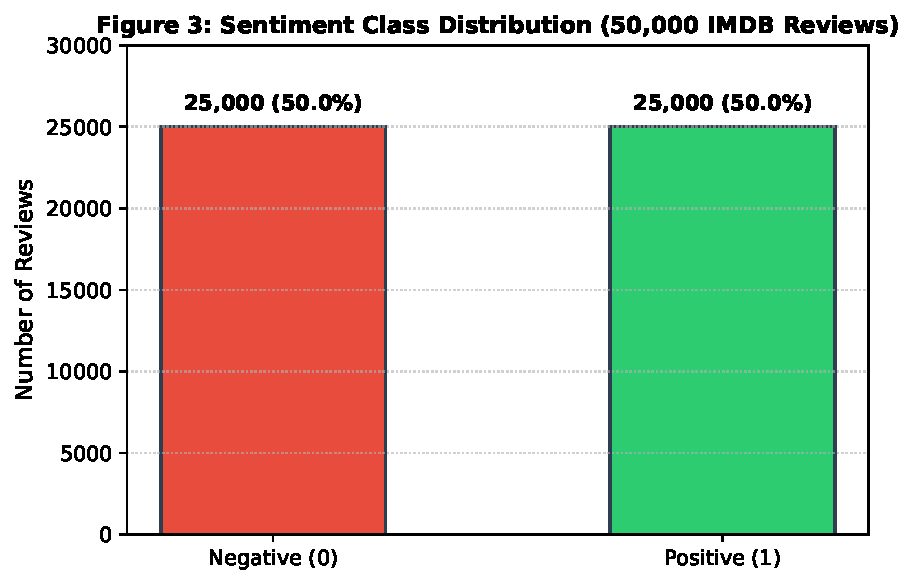
\includegraphics[width=0.60\textwidth]{fig3_class_distribution.pdf}
\caption{Phân bố nhãn lớp trên 50.000 đánh giá, khẳng định dữ liệu hoàn toàn cân bằng.}
\label{fig:eda_class}
\end{figure}

Độ dài của các bài đánh giá được lượng hóa thông qua số lượng từ phân tách bởi khoảng trắng. Như minh họa trong Hình~\ref{fig:eda_length}, phân bố độ dài mang tính lệch phải (positive skewness) rõ rệt. Đánh giá ngắn nhất chỉ có 4 từ, trong khi đánh giá dài nhất lên tới 2.470 từ. Bảng~\ref{tab:length_stats} tổng hợp các chỉ số xu hướng trung tâm và độ phân tán.

\begin{table}[H]
\centering
\begin{tabular}{lr}
\toprule
\textbf{Chỉ số Thống kê} & \textbf{Giá trị Số từ} \\
\midrule
Độ dài Trung bình ($\mu$)         & 231,2 từ \\
Độ dài Trung vị (Median)          & 173,0 từ \\
Độ lệch Chuẩn ($\sigma$)          & 171,3 từ \\
Độ dài Ngắn nhất                  & 4 từ \\
Độ dài Dài nhất                   & 2.470 từ \\
Ngưỡng Cắt chuỗi Cố định ($T_{\max}$) & 250 từ \\
\bottomrule
\end{tabular}
\caption{Các chỉ số thống kê mô tả về độ dài từ vựng trên 50.000 bài đánh giá IMDB.}
\label{tab:length_stats}
\end{table}

\begin{figure}[H]
\centering
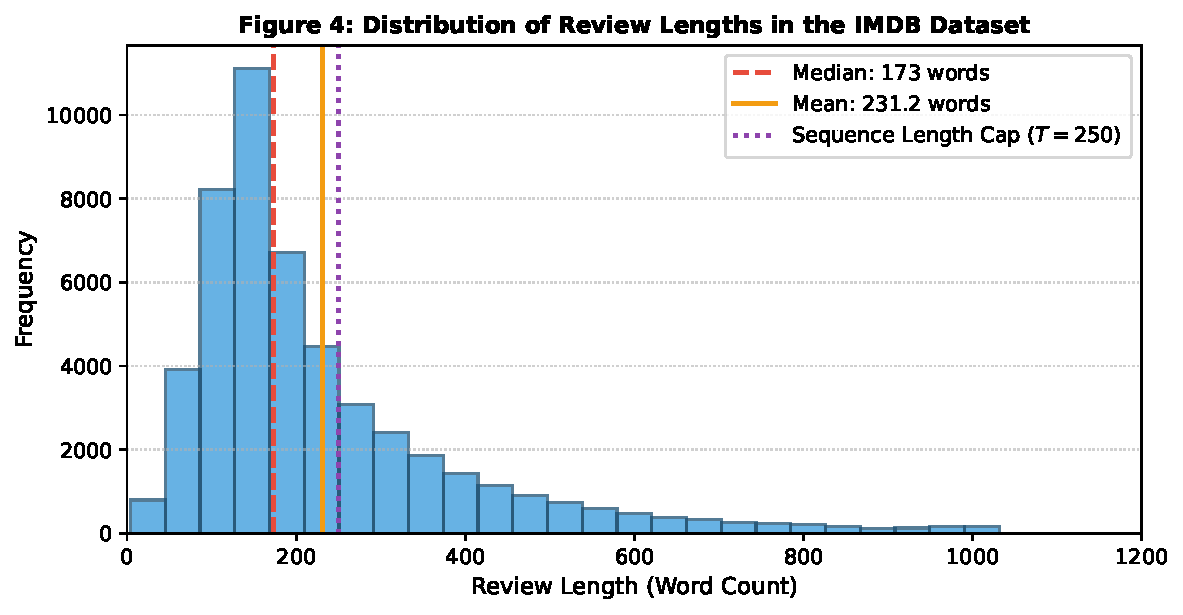
\includegraphics[width=0.78\textwidth]{fig4_review_lengths.pdf}
\caption{Biểu đồ tần suất độ dài các bài đánh giá với các điểm đánh dấu trung vị (173,0 từ), trung bình (231,2 từ) và ngưỡng cắt chuỗi ($T=250$).}
\label{fig:eda_length}
\end{figure}

\subsection{Quy trình Tiền xử lý Văn bản}
Các bài đánh giá thô chứa nhiều mã định dạng HTML thừa (chủ yếu là thẻ xuống dòng \texttt{<br />}), các chữ in hoa và các dấu câu không cần thiết làm phình to kích thước từ điển. Quy trình tiền xử lý áp dụng các bước:
\begin{enumerate}
    \item \textbf{Chuẩn hóa Văn bản:} Chuyển toàn bộ ký tự sang chữ thường, thay thế các thẻ \texttt{<br />} bằng khoảng trắng và loại bỏ các dấu câu thông qua biểu thức chính quy.
    \item \textbf{Tách Token và Xây dựng Từ vựng:} Phân tách văn bản thành các token từ đơn. Tập từ vựng kích thước cố định $|V| = 1.000$ từ có tần suất xuất hiện cao nhất được tạo lập bằng phương thức \texttt{TextVectorization.adapt()}. Chỉ số 0 được dành riêng cho token đệm (\texttt{''}), và chỉ số 1 đại diện cho các từ nằm ngoài từ điển (\texttt{[UNK]}).
    \item \textbf{Chuẩn hóa Độ dài Chuỗi Cố định:} Toàn bộ chuỗi được giới hạn ở ngưỡng $T = 250$ bước thời gian. Các chuỗi ngắn hơn 250 từ sẽ được đệm số 0 ở phía sau (post-padding); các chuỗi dài hơn sẽ bị cắt bỏ sau từ thứ 250.
\end{enumerate}

Bảng~\ref{tab:preproc_params} tổng hợp các tham số cấu hình của quy trình tiền xử lý.

\begin{table}[H]
\centering
\begin{tabular}{llr}
\toprule
\textbf{Tham số} & \textbf{Mô tả Ý nghĩa} & \textbf{Giá trị Cấu hình} \\
\midrule
Kích thước Từ vựng ($|V|$) & Số lượng từ phổ biến nhất được giữ lại & 1.000 \\
Độ dài Chuỗi ($T$)         & Giới hạn bước thời gian hồi quy & 250 tokens \\
Chiến lược Đệm (Padding)   & Giá trị điền cho các chuỗi ngắn & 0 (Post-padding) \\
Token Ngoài Từ điển        & Ký hiệu thay thế từ hiếm gặp & \texttt{[UNK]} (Chỉ số 1) \\
Cơ chế Che mặt nạ (Masking) & Bỏ qua token đệm khi tính BPTT & Bật (\texttt{mask\_zero=True}) \\
\bottomrule
\end{tabular}
\caption{Các tham số cấu hình cho tầng vector hóa và xử lý chuỗi.}
\label{tab:preproc_params}
\end{table}

% =========================================================================
\section{Kiến trúc Mô hình và Cài đặt Thực nghiệm}
\label{sec:architecture}
% =========================================================================

\subsection{Tổng quan Kiến trúc}
Mô hình được xây dựng dưới dạng đồ thị tính toán tuần tự (\texttt{Sequential}) gồm 4 thành phần chức năng: tầng vector hóa văn bản tích hợp, tầng chiếu nhúng từ, khối nơ-ron hồi quy Vanilla và tầng phân loại Dense đầu ra.

\begin{figure}[H]
\centering
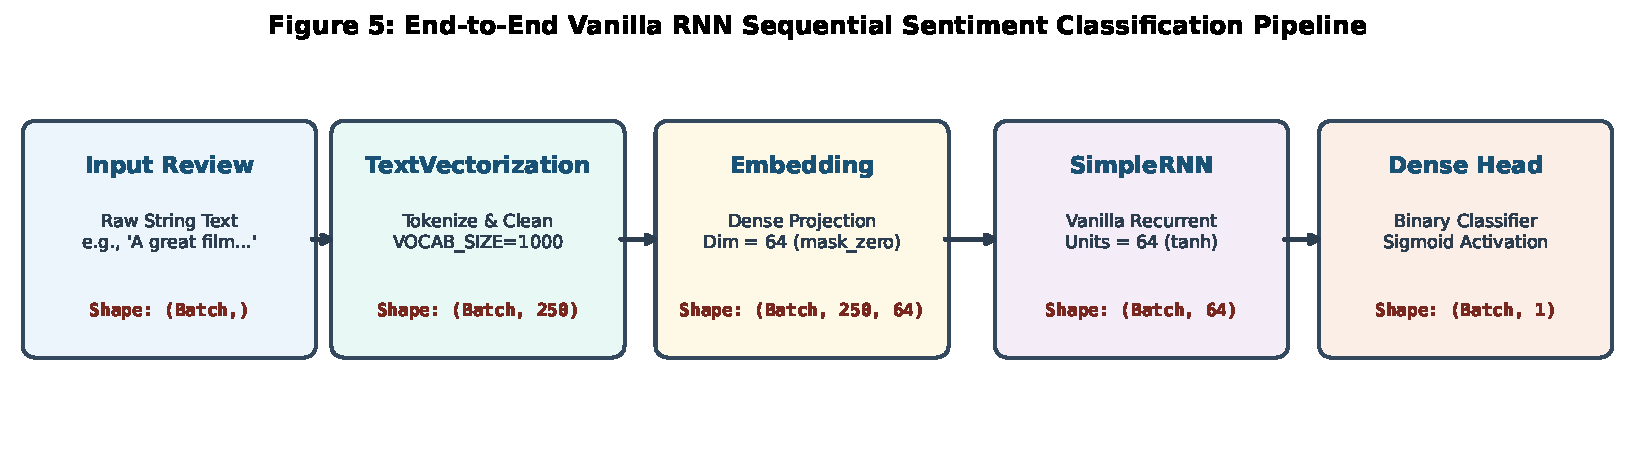
\includegraphics[width=0.95\textwidth]{fig5_model_architecture.pdf}
\caption{Sơ đồ khối chi tiết toàn bộ quy trình phân loại cảm xúc với kích thước tensor qua từng tầng.}
\label{fig:model_arch}
\end{figure}

\subsection{Đặc tả Chi tiết các Tầng}
\begin{itemize}
    \item \textbf{Tầng TextVectorization:} Tiếp nhận mini-batch văn bản thô có dạng $(\text{Batch},)$ và chuyển đổi thành tensor số nguyên 2D biểu diễn chỉ số token có kích thước $(\text{Batch}, 250)$.
    \item \textbf{Tầng Embedding:} Ánh xạ các chỉ số nguyên sang các vector liên tục có số chiều $D = 64$. Với $|V| = 1.000$ từ, tầng này tạo ra tensor đầu ra kích thước $(\text{Batch}, 250, 64)$. Thiết lập \texttt{mask\_zero=True} giúp các tính toán hồi quy phía sau bỏ qua các vị trí đệm.
    \item \textbf{Tầng SimpleRNN:} Triển khai phương trình hồi quy cơ bản (Phương trình~\ref{eq:rnn_hidden}) với $H = 64$ đơn vị ẩn và hàm kích hoạt $\tanh$. Tầng duyệt qua $T = 250$ bước thời gian và trả về vector trạng thái ẩn cuối cùng $h_T$ có kích thước $(\text{Batch}, 64)$.
    \item \textbf{Tầng Dense Đầu ra:} Tầng kết nối đầy đủ với một nơ-ron đơn và hàm kích hoạt sigmoid (Phương trình~\ref{eq:rnn_output}), tính toán xác suất dự đoán $\hat{y} \in [0, 1]$ có dạng $(\text{Batch}, 1)$.
\end{itemize}

\subsection{Số lượng Tham số và Độ phức tạp}
Bảng~\ref{tab:param_counts} liệt kê số lượng tham số chi tiết qua từng tầng. Toàn bộ mô hình có 72.321 tham số có thể huấn luyện ($282,5\text{ KB}$).

\begin{table}[H]
\centering
\begin{tabular}{lllr}
\toprule
\textbf{Tên Tầng} & \textbf{Loại Tầng} & \textbf{Kích thước Tensor Đầu ra} & \textbf{Số Tham số Huấn luyện} \\
\midrule
\texttt{text\_vectorization} & TextVectorization & $(\text{Batch}, 250)$ & 0 \\
\texttt{embedding}          & Embedding         & $(\text{Batch}, 250, 64)$ & 64.000 \\
\texttt{simple\_rnn}        & SimpleRNN         & $(\text{Batch}, 64)$ & 8.256 \\
\texttt{dense}              & Dense             & $(\text{Batch}, 1)$ & 65 \\
\midrule
\textbf{Tổng Tham số}       & \multicolumn{2}{l}{\textbf{72.321 (Tất cả đều được huấn luyện)}} & \textbf{72.321} \\
\bottomrule
\end{tabular}
\caption{Kích thước tensor đầu ra và số lượng tham số huấn luyện qua từng tầng.}
\label{tab:param_counts}
\end{table}

Phép tính tham số được phân rã như sau:
\begin{itemize}
    \item \textbf{Embedding:} $|V| \times D = 1.000 \times 64 = 64.000$.
    \item \textbf{SimpleRNN:} Trọng số đầu vào $W_{xh} = 64 \times 64 = 4.096$; Trọng số hồi quy $W_{hh} = 64 \times 64 = 4.096$; Vector độ lệch $b_h = 64$. Tổng cộng = $4.096 + 4.096 + 64 = 8.256$.
    \item \textbf{Dense Đầu ra:} Trọng số $W_{hy} = 64 \times 1 = 64$; Độ lệch $b_y = 1$. Tổng cộng = $64 + 1 = 65$.
\end{itemize}

% =========================================================================
\section{Thiết lập Thực nghiệm}
\label{sec:setup}
% =========================================================================

\subsection{Cấu hình Huấn luyện và Siêu tham số}
Mô hình được biên dịch với thuật toán tối ưu Adam ở tốc độ học ban đầu $\eta = 10^{-4}$. Mức tốc độ học vừa phải này giúp ngăn chặn hiện tượng bùng nổ gradient qua các bước thời gian hồi quy. Hàm mất mát được sử dụng là Entropy Chéo Nhị phân. Bảng~\ref{tab:hyperparams} ghi nhận toàn bộ các siêu tham số chính.

\begin{table}[H]
\centering
\begin{tabular}{llr}
\toprule
\textbf{Siêu tham số} & \textbf{Định nghĩa / Ý nghĩa} & \textbf{Giá trị Thiết lập} \\
\midrule
Thuật toán Tối ưu      & Bộ tối ưu dựa trên gradient bậc một & Adam \\
Tốc độ Học ($\eta$)    & Hệ số co giãn bước cập nhật trọng số & $1 \times 10^{-4}$ \\
Hàm Mất mát            & Tiêu chuẩn tối ưu hóa & Binary Cross-Entropy \\
Kích thước Batch ($B$) & Số lượng mẫu trong mỗi minibatch & 64 \\
Số Epoch Huấn luyện    & Số lượt duyệt qua toàn bộ tập dữ liệu & 10 \\
Bộ đệm Xáo trộn        & Kích thước vùng đệm ngẫu nhiên hóa & 10.000 \\
Hạt giống Ngẫu nhiên   & Giá trị khởi tạo tái lập kết quả & 42 \\
\bottomrule
\end{tabular}
\caption{Thiết lập các siêu tham số cho quy trình huấn luyện.}
\label{tab:hyperparams}
\end{table}

\subsection{Môi trường Phần cứng và Phần mềm}
Mọi thực nghiệm tính toán được tiến hành trên nền tảng Linux x86\_64 (hệ điều hành Ubuntu 24.04 LTS). Hệ thống phần mềm sử dụng Python 3.12.3, TensorFlow 2.21.0, Keras 3.15.1, NumPy 2.5.3, Scikit-Learn 1.9.1, và Matplotlib 3.11.2. Môi trường tính toán vận hành trên CPU được tối ưu hóa tập lệnh AVX2.

\subsection{Các Thang đo Đánh giá}
Hiệu năng của mô hình trên tập kiểm thử ($D_{\text{test}}$) được đo lường thông qua các chỉ số thống kê chuẩn mực:
\begin{itemize}
    \item \textbf{Độ chính xác Toàn thể (Accuracy):} Tỷ lệ các mẫu được dự đoán chính xác trên tổng số mẫu:
    \begin{equation}
    \text{Accuracy} = \frac{TP + TN}{TP + TN + FP + FN}
    \end{equation}
    \item \textbf{Độ chính xác Dương tính (Precision):} Tỷ lệ mẫu thực sự tích cực trên tổng số mẫu được mô hình dự đoán là tích cực:
    \begin{equation}
    \text{Precision} = \frac{TP}{TP + FP}
    \end{equation}
    \item \textbf{Độ bao phủ / Độ nhạy (Recall):} Tỷ lệ mẫu tích cực được mô hình nhận diện thành công trên toàn bộ số mẫu tích cực thực tế:
    \begin{equation}
    \text{Recall} = \frac{TP}{TP + FN}
    \end{equation}
    \item \textbf{Điểm $F_1$ ($F_1$-Score):} Trung bình điều hòa giữa Precision và Recall:
    \begin{equation}
    F_1 = 2 \times \frac{\text{Precision} \times \text{Recall}}{\text{Precision} + \text{Recall}}
    \end{equation}
    \item \textbf{ROC-AUC:} Diện tích dưới đường cong Đặc trưng Hoạt động của Bộ thu, thể hiện khả năng phân tách giữa hai lớp nhãn tại mọi ngưỡng quyết định.
\end{itemize}

% =========================================================================
\section{Kết quả Thực nghiệm và Tiến trình Huấn luyện}
\label{sec:results}
% =========================================================================

\subsection{Đường cong Tiến trình Huấn luyện}
Mô hình Vanilla RNN được huấn luyện qua 10 epoch hoàn chỉnh. Bảng~\ref{tab:epoch_progression} trình bày chi tiết các số liệu thực nghiệm đo đạc được tại mỗi epoch.

\begin{table}[H]
\centering
\begin{tabular}{rrrrr}
\toprule
\textbf{Epoch} & \textbf{Loss Huấn luyện ($\mathcal{L}_{\text{train}}$)} & \textbf{Độ chính xác Train ($\%$)} & \textbf{Loss Kiểm chuẩn ($\mathcal{L}_{\text{val}}$)} & \textbf{Độ chính xác Val ($\%$)} \\
\midrule
1  & 0,6351 & 63,19\% & 0,5301 & 77,74\% \\
2  & 0,4691 & 79,44\% & 0,5464 & 72,16\% \\
3  & 0,4088 & 82,83\% & 0,4129 & 82,36\% \\
4  & 0,3758 & 84,51\% & 0,3815 & 83,57\% \\
5  & 0,3555 & 85,19\% & 0,4084 & 82,85\% \\
6  & 0,3419 & 86,00\% & 0,3819 & 83,15\% \\
7  & 0,3329 & 86,15\% & 0,3782 & 83,19\% \\
8  & 0,3261 & 86,52\% & 0,4031 & 83,52\% \\
9  & 0,3181 & 86,77\% & 0,3628 & 84,04\% \\
10 & 0,3117 & 86,92\% & 0,3723 & 83,66\% \\
\bottomrule
\end{tabular}
\caption{Bảng theo dõi các số liệu tiến trình huấn luyện qua 10 epoch trên 25.000 mẫu tập train và validation.}
\label{tab:epoch_progression}
\end{table}

Hình~\ref{fig:curve_loss} và Hình~\ref{fig:curve_acc} minh họa quỹ đạo giảm thiểu hàm mất mát và sự tăng trưởng của độ chính xác qua các epoch.

\begin{figure}[H]
\centering
\begin{subfigure}[b]{0.48\textwidth}
    \centering
    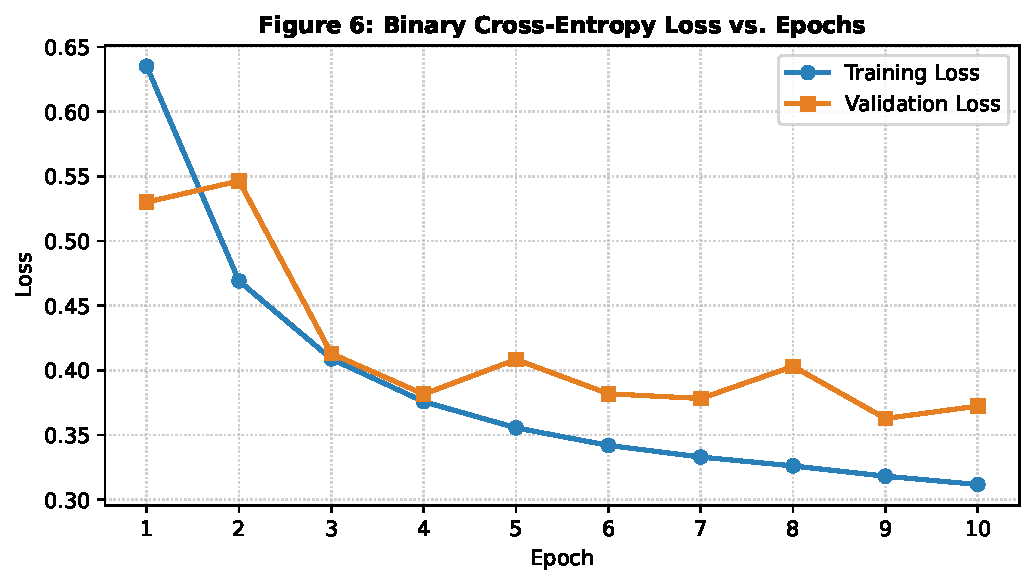
\includegraphics[width=\textwidth]{fig6_training_loss.pdf}
    \caption{Hàm mất mát Binary Cross-Entropy qua từng Epoch.}
    \label{fig:curve_loss}
\end{subfigure}
\hfill
\begin{subfigure}[b]{0.48\textwidth}
    \centering
    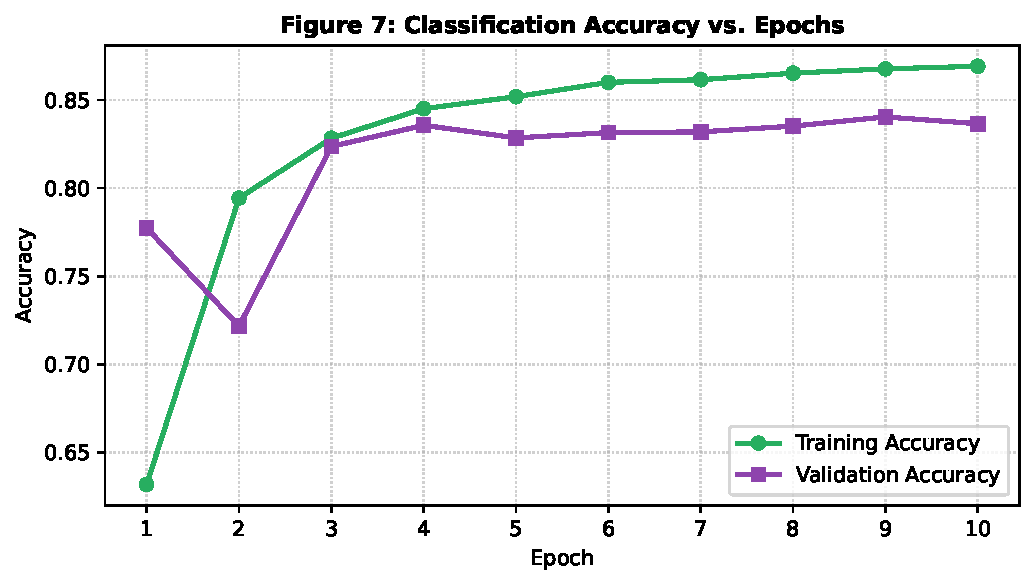
\includegraphics[width=\textwidth]{fig7_training_accuracy.pdf}
    \caption{Độ chính xác phân loại qua từng Epoch.}
    \label{fig:curve_acc}
\end{subfigure}
\caption{Đường cong huấn luyện thực nghiệm cho thấy tốc độ hội tụ nhanh ở các epoch đầu và đi vào trạng thái ổn định từ epoch 5 đến epoch 10.}
\label{fig:training_curves}
\end{figure}

Các đồ thị cho thấy khả năng học rất nhanh trong các epoch từ 1 đến 4: mất mát huấn luyện giảm mạnh từ 0,6351 xuống 0,3758, và độ chính xác kiểm chuẩn tăng vọt từ 77,74\% lên 83,57\%. Sau epoch 6, mất mát huấn luyện tiếp tục giảm từ từ xuống 0,3117, trong khi mất mát kiểm chuẩn dao động ổn định trong khoảng $0,3628$--$0,3782$, báo hiệu mô hình đã tiệm cận mức dung lượng biểu diễn tối ưu.

\subsection{Đánh giá Chung cuộc trên Tập Kiểm thử}
Đánh giá trên 25.000 mẫu đánh giá độc lập của tập kiểm thử mang lại các chỉ số thống nhất. Như được nêu rõ trong Bảng~\ref{tab:test_metrics}, mô hình đạt độ chính xác toàn thể 83,66\% và chỉ số ROC-AUC đạt 0,9193.

\begin{table}[H]
\centering
\begin{tabular}{llr}
\toprule
\textbf{Chỉ số Thang đo} & \textbf{Công thức / Định nghĩa} & \textbf{Kết quả Kiểm thử} \\
\midrule
Loss Kiểm thử ($\mathcal{L}_{\text{test}}$) & Binary Cross-Entropy & 0,3723 \\
Độ chính xác (Accuracy)                     & Số mẫu đúng / Tổng số mẫu & \textbf{83,66\%} \\
Độ chính xác Dương tính (Precision)         & $TP / (TP + FP)$ & \textbf{80,00\%} \\
Độ bao phủ / Nhạy (Recall)                  & $TP / (TP + FN)$ & \textbf{89,69\%} \\
Điểm $F_1$ ($F_1$-Score)                    & Trung bình điều hòa Precision và Recall & \textbf{84,57\%} \\
Chỉ số ROC-AUC                              & Diện tích dưới đường cong ROC & \textbf{0,9193} \\
\bottomrule
\end{tabular}
\caption{Đánh giá định lượng toàn diện trên tập kiểm thử gồm 25.000 đánh giá.}
\label{tab:test_metrics}
\end{table}

Ma trận Nhầm lẫn (Hình~\ref{fig:cm_heatmap}) chỉ ra rằng mô hình đã phát hiện chính xác 11.196 mẫu tích cực (True Positives, chiếm 89,6\% lớp tích cực) và 9.718 mẫu tiêu cực (True Negatives, chiếm 77,7\% lớp tiêu cực). Mô hình gặp phải 2.799 trường hợp Dương tính giả (False Positives - mẫu tiêu cực bị phân loại nhầm thành tích cực) và 1.287 trường hợp Âm tính giả (False Negatives - mẫu tích cực bị phân loại nhầm thành tiêu cực).

\begin{figure}[H]
\centering
\begin{subfigure}[b]{0.48\textwidth}
    \centering
    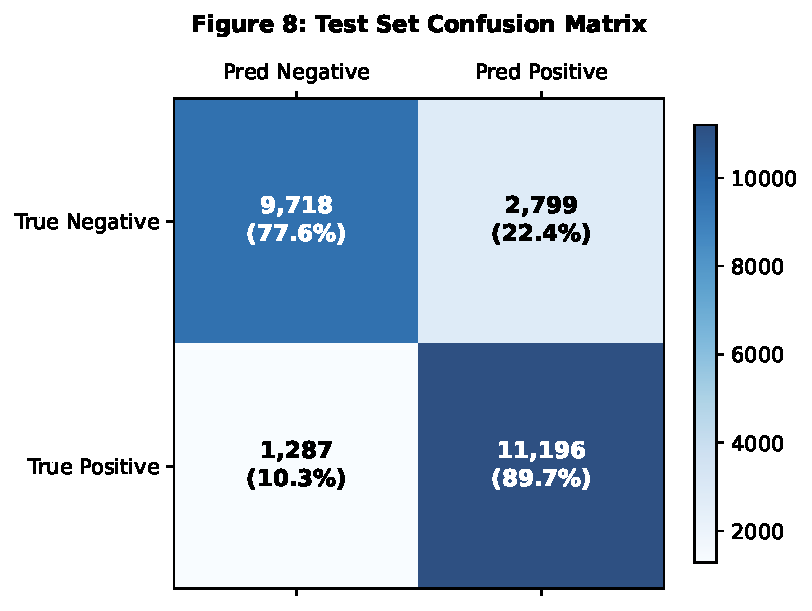
\includegraphics[width=\textwidth]{fig8_confusion_matrix.pdf}
    \caption{Ma trận Nhầm lẫn trên 25.000 đánh giá kiểm thử.}
    \label{fig:cm_heatmap}
\end{subfigure}
\hfill
\begin{subfigure}[b]{0.48\textwidth}
    \centering
    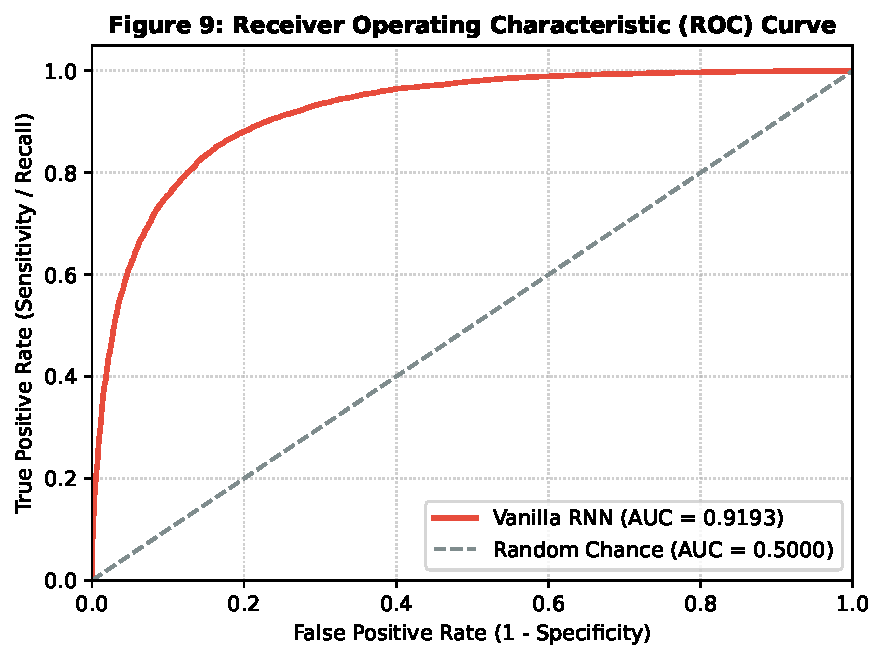
\includegraphics[width=\textwidth]{fig9_roc_curve.pdf}
    \caption{Đường cong ROC với chỉ số AUC = 0,9193.}
    \label{fig:roc_curve}
\end{subfigure}
\caption{Các biểu đồ đánh giá chẩn đoán phân loại trên tập dữ liệu kiểm thử.}
\label{fig:diagnostics}
\end{figure}

Đường cong ROC (Hình~\ref{fig:roc_curve}) uốn cong mạnh mẽ về góc trên bên trái $(0, 1)$, khẳng định năng lực phân tách lớp xuất sắc trên một dải rộng các ngưỡng quyết định vận hành.

\subsection{Dự đoán trên Mẫu Thực tế}
Bảng~\ref{tab:sample_preds} trình bày các kết quả đánh giá suy luận định tính được trích xuất trực tiếp từ tập kiểm thử, đối chiếu các phân loại chính xác với độ tin cậy cao cùng các trường hợp lỗi điển hình.

\begin{table}[H]
\centering
\small
\begin{tabular}{p{7.2cm}cccp{2.6cm}}
\toprule
\textbf{Đoạn Trích Đánh giá} & \textbf{Thực} & \textbf{$\hat{y}$ (Xác suất)} & \textbf{Đoán} & \textbf{Phân loại Kết quả} \\
\midrule
\textit{``After seeing 'Break a Leg' in Vancouver at the release party I thought it was a very enjoyable film. I had a few outright belly...''} & 1 & 0,9666 & 1 & \textbf{Dương tính Thật (TP)} (Độ tin cậy rất cao) \\
\midrule
\textit{``I enjoyed Longstreet, which followed in the steps of Raymond Burr's successful Ironside TV series and was intended to give it c...''} & 1 & 0,8326 & 1 & \textbf{Dương tính Thật (TP)} (Độ tin cậy tốt) \\
\midrule
\textit{``Wow, here it finally is; the action ``movie'' without action. In a real low-budget setting (don't miss the hilarious flying sauce...''} & 0 & 0,0214 & 0 & \textbf{Âm tính Thật (TN)} (Độ tin cậy rất cao) \\
\midrule
\textit{``"Sir" John Gielgud must have become senile to star in a mess of a movie like this one.; This is one of those films, I suppose, ...''} & 0 & 0,2258 & 0 & \textbf{Âm tính Thật (TN)} (Bác bỏ rõ ràng) \\
\midrule
\textit{``"Congo" is based on the best-selling novel by Michael Crichton, which I thought lacked Crichton's usual charm, smart characters...''} & 0 & 0,9216 & 1 & \textbf{Dương tính Giả (FP)} (Lỗi phân loại nhầm) \\
\midrule
\textit{``'Identity\dots I am part of my surroundings and I became separate from them and it's being able to make those differentiati...''} & 1 & 0,3417 & 0 & \textbf{Âm tính Giả (FN)} (Lỗi phân loại nhầm) \\
\bottomrule
\end{tabular}
\caption{Các bài đánh giá tiêu biểu và kết quả dự đoán tạo ra bởi mô hình Vanilla RNN trên tập kiểm thử.}
\label{tab:sample_preds}
\end{table}

\subsection{Phân tích Lỗi Sai}
Phân tích lỗi định tính đối với các trường hợp phân loại sai trong Bảng~\ref{tab:sample_preds} làm sáng tỏ hai cơ chế gây lỗi ngôn ngữ chính:
\begin{enumerate}
    \item \textbf{Dương tính Giả trên Phê bình Thâm trầm có Từ khóa Tích cực:} Trong bài đánh giá phim \textit{Congo}, người viết đề cập rằng bộ phim dựa trên một cuốn tiểu thuyết bán chạy (\textit{``best-selling novel''}) và nhắc tới các yếu tố \textit{``charm, smart characters''}, mặc dù được đặt trong ngữ cảnh phủ định (\textit{``which I thought lacked\dots''}). Vì Vanilla SimpleRNN nén toàn bộ chuỗi vào vector 64 chiều, các từ khóa tích cực mạnh xuất hiện ở đầu chuỗi đã áp đảo trạng thái ẩn cuối cùng, lấn át thông điệp phê bình tiêu cực ở phía sau.
    \item \textbf{Âm tính Giả trên Diễn đạt Triết lý / Trừu tượng:} Bài đánh giá tích cực của bộ phim \textit{Identity} mở đầu bằng văn phong triết lý với nhiều từ vựng học thuật không nằm trong danh mục 1.000 từ phổ biến (khiến chúng bị ánh xạ thành token \texttt{[UNK]}). Do thiếu các dấu hiệu cảm xúc tích cực nổi bật ở phần mở đầu, trạng thái hồi quy không tích lũy đủ độ kích hoạt dương tính.
\end{enumerate}

% =========================================================================
\section{Thảo luận}
\label{sec:discussion}
% =========================================================================

\subsection{Diễn giải Động lực Huấn luyện}
Tiến trình thực nghiệm chứng minh rằng ngay cả một mô hình Vanilla RNN kích thước nhỏ gọn (72.321 tham số) vẫn có thể đạt độ chính xác tổng quát hóa 83,66\% trên ngôn ngữ tự nhiên đời thường vốn phức tạp. Chênh lệch giữa độ chính xác huấn luyện (86,92\%) và kiểm chuẩn (83,66\%) sau 10 epoch là tương đối nhỏ ($\approx 3,26\%$), chứng tỏ mô hình không bị rơi vào hiện tượng quá khớp (overfitting) nghiêm trọng. Sự ổn định này xuất phát từ:
\begin{itemize}
    \item Quy mô từ vựng bảo thủ ($|V| = 1.000$), đóng vai trò như một cơ chế điều hòa (regularization) ngầm định nhằm loại bỏ các từ hiếm và nhiễu.
    \item Tốc độ học thấp ($\eta = 10^{-4}$), giúp ngăn ngừa các bước nhảy tham số quá trớn gây mất ổn định ma trận hồi quy $W_{hh}$.
    \item Cơ chế che mặt nạ giá trị 0 (\texttt{mask\_zero=True}), giúp ngăn các token đệm làm suy giảm độ chính xác của các trạng thái ẩn trên các câu có độ dài ngắn.
\end{itemize}

\subsection{Tác động của các Cấu hình Siêu tham số}
\begin{itemize}
    \item \textbf{Quy mô Từ vựng ($|V| = 1.000$):} Mặc dù giúp giảm tải tính toán, việc giới hạn từ điển ở 1.000 từ buộc nhiều từ vựng giàu sắc thái biểu cảm (như ``magnificent'', ``dreadful'', ``masterpiece'') phải chuyển thành token \texttt{[UNK]}. Việc mở rộng $|V|$ lên 10.000 từ sẽ nâng cao độ phân giải ngữ nghĩa, nhưng sẽ làm tăng kích thước bảng nhúng từ ($10.000 \times 64 = 640.000$ tham số).
    \item \textbf{Độ dài Chuỗi ($T = 250$):} Cắt chuỗi ở 250 từ là phù hợp với đa số đánh giá (trung vị là 173 từ), nhưng sẽ làm mất đi các câu tổng kết ở đoạn cuối của các bài viết dài (vốn có thể dài tới 2.470 từ).
    \item \textbf{Số chiều Ẩn ($H = 64$):} 64 đơn vị ẩn cung cấp vừa đủ năng lực biểu diễn cho bài toán phân loại cảm xúc nhị phân trong khi vẫn đảm bảo tốc độ huấn luyện cao trên kiến trúc CPU.
\end{itemize}

\subsection{Những Giới hạn Cố hữu của Kiến trúc Vanilla RNN}
Bất chấp hiệu năng ấn tượng, kiến trúc Vanilla RNN vẫn bộc lộ các rào cản nội tại:
\begin{itemize}
    \item \textbf{Triệt tiêu Đạo hàm trên Ngữ cảnh Tầm xa:} Như đã chứng minh giải tích tại Phương trình~\ref{eq:jacobian_product}, gradient của Vanilla RNN suy giảm theo hàm mũ khi truyền ngược qua 250 bước thời gian. Do đó, các từ ngữ ở đầu một bài đánh giá dài gần như không còn tác động tới việc cập nhật trọng số so với các từ ở cuối bài.
    \item \textbf{Nút thắt Thông tin (Information Bottleneck):} Việc nén toàn bộ văn bản có độ dài bất kỳ vào một vector cố định $h_T \in \mathbb{R}^{64}$ buộc mạng phải liên tục loại bỏ các thông tin chi tiết trong quá khứ.
    \item \textbf{Thiếu Cơ chế Cổng (Gating):} Sự vắng mặt của các đường dẫn bộ nhớ cộng tính khiến mạng gặp khó khăn trong việc lưu giữ một cảm xúc nhất quán qua các mệnh đề phụ xen ngang.
\end{itemize}

\subsection{So sánh với Phương pháp Truyền thống}
So với mô hình truyền thống TF-IDF kết hợp Hồi quy Logistic (thường đạt khoảng 86--88\% độ chính xác trên IMDB), kết quả 83,66\% của mô hình Vanilla SimpleRNN này hơi thấp hơn đôi chút. Sự chênh lệch này giải thích được hoàn toàn do sự giới hạn từ điển (1.000 từ so với 10.000+ n-gram trong TF-IDF) và ảnh hưởng của hiện tượng triệt tiêu đạo hàm. Dẫu vậy, RNN tạo tiền đề học sâu khả vi khép kín, có thể mở rộng xử lý chuỗi trực tiếp mà không cần thiết kế đặc trưng thủ công.

% =========================================================================
\section{Kết luận và Hướng Phát triển}
\label{sec:conclusion}
% =========================================================================

\subsection{Tổng kết Kết quả Nghiên cứu}
Trong nghiên cứu này, một hệ thống phân loại Mạng Nơ-ron Hồi quy Cơ bản (Vanilla SimpleRNN) đã được thiết kế, cài đặt và kiểm chứng thực nghiệm hoàn chỉnh trên tập dữ liệu chuẩn IMDB gồm 50.000 bài đánh giá. Sử dụng TensorFlow và Keras, nhóm nghiên cứu đã xây dựng một đường ống hợp nhất có khả năng tách từ trực tiếp từ văn bản thô, ánh xạ sang không gian nhúng liên tục 64 chiều, mô hình hóa các mối phụ thuộc tuần tự và thực hiện phân loại nhị phân.

Sau 10 epoch huấn luyện, mô hình đạt sự hội tụ vững chắc với độ chính xác huấn luyện 86,92\% và độ chính xác kiểm thử chung cuộc đạt 83,66\%. Phân tích chẩn đoán toàn diện ghi nhận điểm $F_1$ đạt 84,57\% và chỉ số ROC-AUC đạt 0,9193. Các phân tích ma trận nhầm lẫn và khảo sát định tính chỉ ra rằng các lỗi phân loại chủ yếu xuất phát từ giới hạn độ dài từ điển và sự suy giảm thông tin ngữ cảnh trên chuỗi dài.

\subsection{Hướng Nghiên cứu và Cải tiến Tương lai}
Nhằm khắc phục các giới hạn thực nghiệm và lý thuyết đã được chỉ ra, các hướng phát triển tiếp theo bao gồm:
\begin{enumerate}
    \item \textbf{Kiến trúc Hồi quy có Cổng (Gated Architectures):} Triển khai mạng LSTM (Long Short-Term Memory) hoặc GRU (Gated Recurrent Unit) để thiết lập các xa lộ gradient cộng tính, giải quyết triệt để vấn đề triệt tiêu đạo hàm trên chuỗi dài.
    \item \textbf{Biểu diễn Vector Tiền Huấn luyện:} Khởi tạo tầng nhúng từ bằng các vector học chuyển giao như GloVe (Global Vectors for Word Representation) hoặc FastText để tận dụng tri thức ngữ nghĩa từ các kho ngữ liệu web khổng lồ.
    \item \textbf{Mô hình hóa Hai chiều (Bidirectional):} Sử dụng mô hình RNN hai chiều (\texttt{Bidirectional(SimpleRNN)}) để khai thác đồng thời cả ngữ cảnh quá khứ và tương lai.
    \item \textbf{Cơ chế Chú ý và Transformers:} Tích hợp cơ chế tự chú ý (Self-Attention) để loại bỏ nút thắt cổ chai của quá trình tuần tự, cho phép tương tác trực tiếp giữa các cặp từ bất kể khoảng cách vị trí.
\end{enumerate}

% =========================================================================
\begin{thebibliography}{99}
% =========================================================================

\bibitem{maas2011learning}
A.~L. Maas, R.~E. Daly, P.~T. Pham, D.~Huang, A.~Y. Ng, and C.~Potts,
\newblock ``Learning word vectors for sentiment analysis,''
\newblock in \emph{Proceedings of the 49th Annual Meeting of the Association for Computational Linguistics: Human Language Technologies}, pp. 142--150, 2011.

\bibitem{rumelhart1986learning}
D.~E. Rumelhart, G.~E. Hinton, and R.~J. Williams,
\newblock ``Learning representations by back-propagating errors,''
\newblock \emph{Nature}, vol. 323, no. 6088, pp. 533--536, 1986.

\bibitem{werbos1990backpropagation}
P.~J. Werbos,
\newblock ``Backpropagation through time: what it does and how to do it,''
\newblock \emph{Proceedings of the IEEE}, vol. 78, no. 10, pp. 1550--1560, 1990.

\bibitem{bengio1994learning}
Y.~Bengio, P.~Simard, and P.~Frasconi,
\newblock ``Learning long-term dependencies with gradient descent is difficult,''
\newblock \emph{IEEE Transactions on Neural Networks}, vol. 5, no. 2, pp. 157--166, 1994.

\bibitem{pascanu2013difficulty}
R.~Pascanu, T.~Mikolov, and Y.~Bengio,
\newblock ``On the difficulty of training recurrent neural networks,''
\newblock in \emph{International Conference on Machine Learning (ICML)}, pp. 1310--1318, 2013.

\bibitem{chollet2021deep}
F.~Chollet,
\newblock \emph{Deep Learning with Python},
\newblock Simon and Schuster, 2nd ed., 2021.

\bibitem{kingma2014adam}
D.~P. Kingma and J.~Ba,
\newblock ``Adam: A method for stochastic optimization,''
\newblock in \emph{International Conference on Learning Representations (ICLR)}, 2015.

\end{thebibliography}

\newpage
% =========================================================================
\appendix
\section{Phụ lục: Mã nguồn Cài đặt}
\label{sec:appendix}
% =========================================================================

\subsection{Nạp Dữ liệu và Thiết lập Đường ống tf.data}
Đoạn mã sau thể hiện quá trình đọc tệp CSV cục bộ, ánh xạ nhãn cảm xúc và cấu hình đường ống nạp dữ liệu nạp trước (prefetching).

\begin{lstlisting}[language=Python, caption={Quy trình nạp dữ liệu và khởi tạo đường ống tf.data.}]
import os
import numpy as np
import pandas as pd
import tensorflow as tf

# Đọc tập dữ liệu CSV cục bộ
df = pd.read_csv("Vanilla RNN/datasets/IMDB Dataset.csv")
df['label'] = df['sentiment'].map({'positive': 1, 'negative': 0}).astype(np.int32)

# Xáo trộn và phân chia tập dữ liệu tỷ lệ 50/50 Train và Test
df_shuffled = df.sample(frac=1.0, random_state=42).reset_index(drop=True)
train_texts = df_shuffled['review'].iloc[:25000].values
train_labels = df_shuffled['label'].iloc[:25000].values
test_texts  = df_shuffled['review'].iloc[25000:].values
test_labels = df_shuffled['label'].iloc[25000:].values

# Xây dựng đường ống nạp dữ liệu hiệu năng cao với tf.data
BUFFER_SIZE = 10000
BATCH_SIZE = 64

train_ds = (
    tf.data.Dataset.from_tensor_slices((train_texts, train_labels))
    .shuffle(BUFFER_SIZE, seed=42)
    .batch(BATCH_SIZE)
    .prefetch(tf.data.AUTOTUNE)
)

test_ds = (
    tf.data.Dataset.from_tensor_slices((test_texts, test_labels))
    .batch(BATCH_SIZE)
    .prefetch(tf.data.AUTOTUNE)
)
\end{lstlisting}

\subsection{Tiền xử lý và Xây dựng Kiến trúc Vanilla SimpleRNN}
Đoạn mã định nghĩa hàm chuẩn hóa văn bản tùy biến, tầng vector hóa và cấu trúc mô hình tuần tự.

\begin{lstlisting}[language=Python, caption={Định nghĩa mô hình với các tầng TextVectorization, Embedding, SimpleRNN và Dense.}]
import re
import string

VOCAB_SIZE = 1000
SEQ_LEN = 250

def custom_standardizer(input_text):
    lowercase = tf.strings.lower(input_text)
    clean_html = tf.strings.regex_replace(lowercase, '<br />', ' ')
    return tf.strings.regex_replace(clean_html, f'[{re.escape(string.punctuation)}]', '')

encoder = tf.keras.layers.TextVectorization(
    max_tokens=VOCAB_SIZE,
    standardize=custom_standardizer,
    output_mode='int',
    output_sequence_length=SEQ_LEN
)
encoder.adapt(train_texts)

model = tf.keras.Sequential([
    encoder,
    tf.keras.layers.Embedding(
        input_dim=len(encoder.get_vocabulary()),
        output_dim=64,
        mask_zero=True
    ),
    tf.keras.layers.SimpleRNN(64),
    tf.keras.layers.Dense(1, activation='sigmoid')
], name="Vanilla_SimpleRNN_Classifier")

model.compile(
    loss=tf.keras.losses.BinaryCrossentropy(from_logits=False),
    optimizer=tf.keras.optimizers.Adam(learning_rate=1e-4),
    metrics=['accuracy']
)
\end{lstlisting}

\subsection{Quy trình Huấn luyện và Đánh giá Mô hình}
Đoạn mã thực thi quá trình huấn luyện và đánh giá định lượng trên tập kiểm thử:

\begin{lstlisting}[language=Python, caption={Vòng lặp huấn luyện và đánh giá thang đo.}]
# Huấn luyện mô hình qua 10 epoch
history = model.fit(
    train_ds,
    epochs=10,
    validation_data=test_ds,
    shuffle=False
)

# Đánh giá định lượng trên tập kiểm thử
test_loss, test_acc = model.evaluate(test_ds, verbose=0)
print(f"Test Loss: {test_loss:.4f} | Test Accuracy: {test_acc*100:.2f}%")

# Thực hiện suy luận dự đoán trên chuỗi văn bản bất kỳ
sample_text = "This movie was fantastic and I loved every minute of it!"
prediction = model.predict(tf.constant([sample_text]), verbose=0)[0][0]
sentiment = "Tích cực" if prediction > 0.5 else "Tiêu cực"
print(f"Dự đoán: {sentiment} ({prediction:.4f})")
\end{lstlisting}

\end{document}
